\chapter{The LHC and ATLAS Experiment}
\section{The Large Hadron Collider}
\section{The ATLAS Detector}
\subsection{Magnet System}
In order to measure the charge and momentum of particles in the detector, a magnetic field is induced. Through the curvature of a charged particle track, the charge to mass ratio can be derived. The sign of the charge is determined from the direction of the track.

The magnet system in ATLAS is a hybrid system comprised of four superconducting magnets: a central solenoid, a barrel toroid, and two end-cap toroids. The barrel toroids define the dimensions of the system, extending 26 m along the beam axis, and has an outer diameter of 22 m
\cite{magnet-system-tdr}. A schematic of the components magnet system is shown in Figure \ref{fig:magnetSystem}.

% Insert picture
\begin{figure}
    \centering
    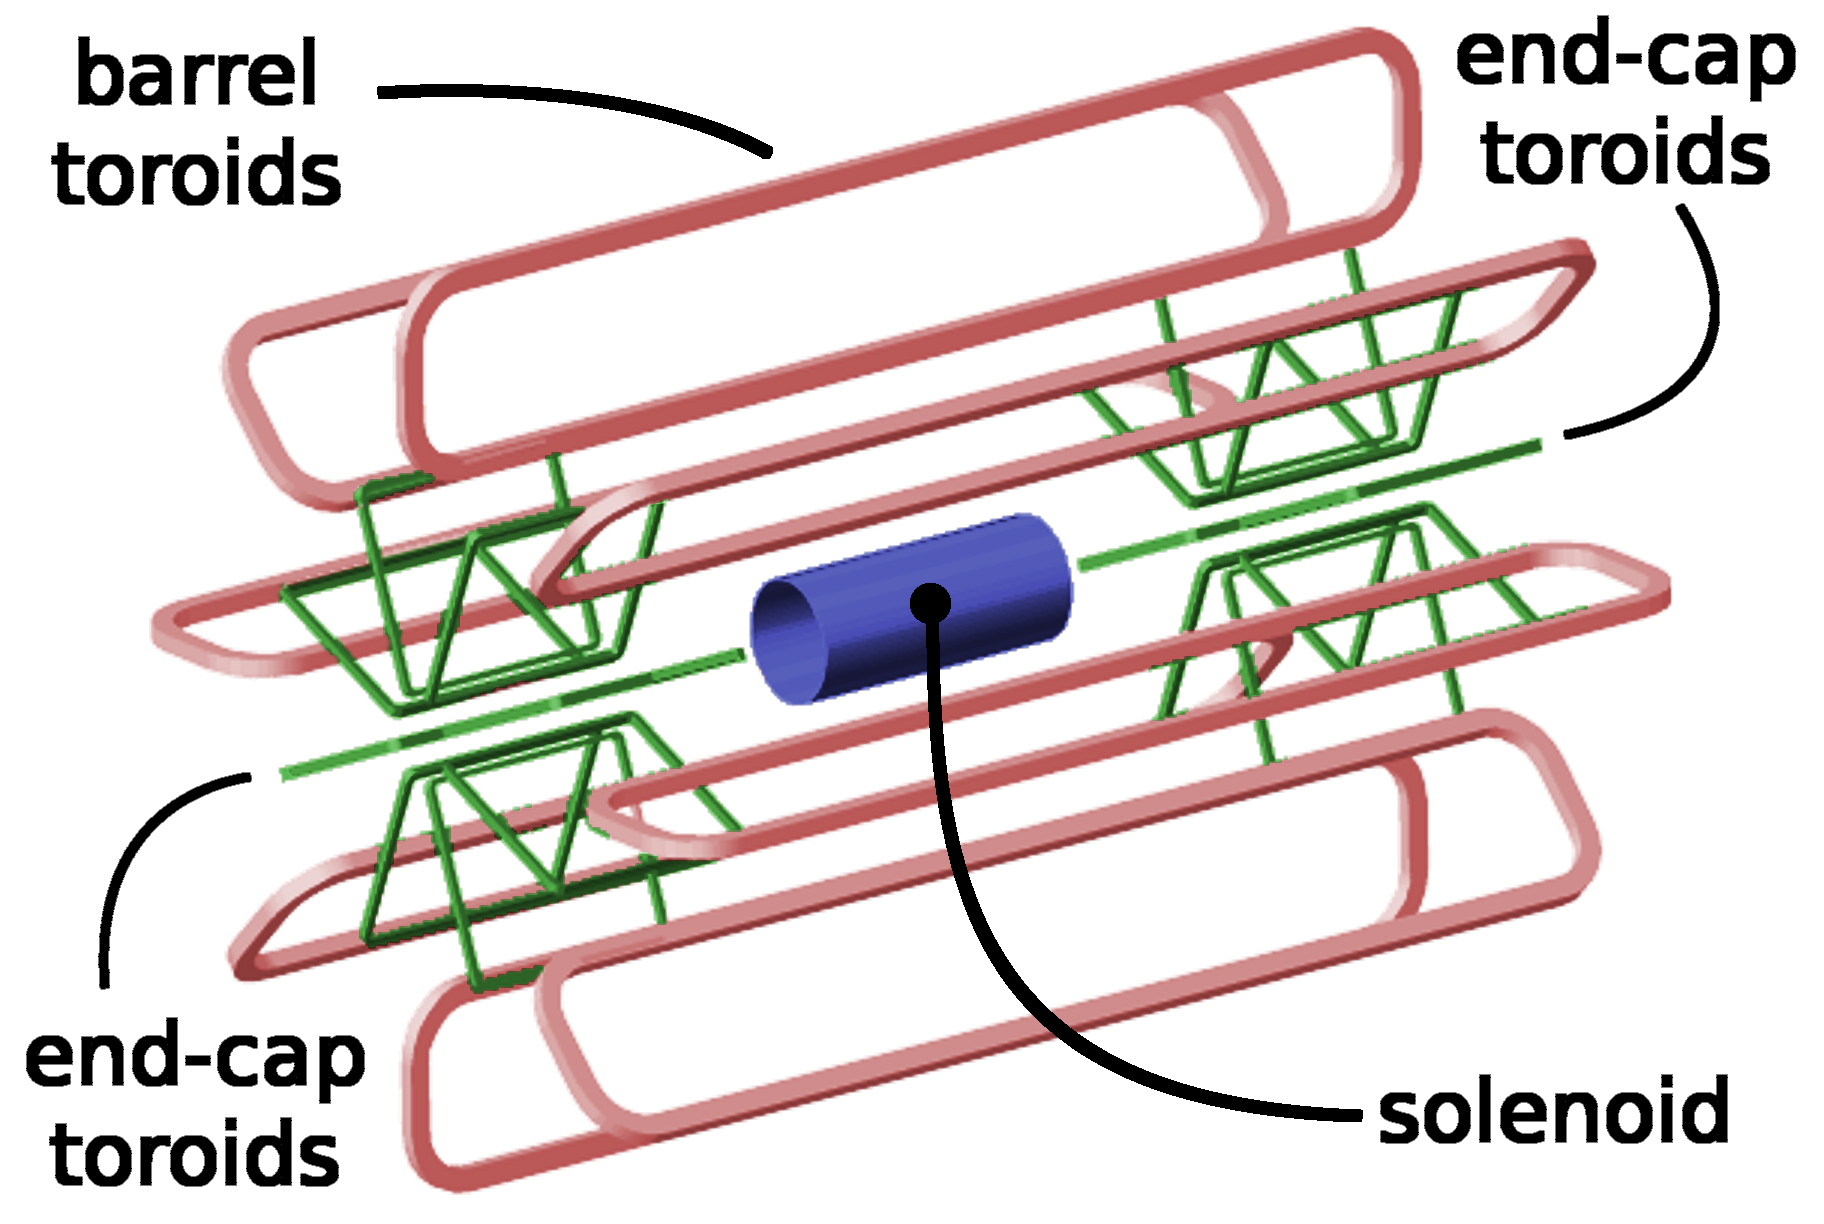
\includegraphics[width=.9\textwidth]{chapters/chapter2_experiment/images/magnetSystems.png}
    \caption{A schematic of the components of the magnet system in the ATLAS detector \cite{magnet-schematic}}
    \label{fig:magnetSystem}
\end{figure}

\begin{itemize}
    \item The central solenoid provides a 2 Tesla magnetic field. It is fitted between the \gls{ID} and the \gls{EM} calorimeter. Arising from a solenoid, this field is axially symmetric, and causes curvature in charged particles as they move through the \gls{ID}. In order to minimize material before the calorimeters, it was designed to be thin, a single-layer coil wound with 1173 turns with Al-stabilized Nb/Ti conductor. It covers a length of 5.3 m along the beam axis and has an outer diameter of 2.63 m\cite{central-solenoid}.

    \item The barrel toroid is made up of eight coils of a flat racetrack shape, which provide a symmetric radial field toward the beam axis, with a peak of 3.9 T \cite{barrel-toroid}. The two end-cap toroids are also composed of eight coils, with a length of 5 m, outer diameter of 10.7 m and an inner bore of 1.65 m, and providing a peak 4.1 T field. The end-cap toroids are inserted into the barrel toroid and line up with the center solenoid. The three-toroid design was chosen over a single toroid to maintain easy access to the core of the detector \cite{endcap-toroid}. Together the toroids provide a magnetic field to the muon system, causing curvature in the muon trajectory.
\end{itemize}


\subsection{Inner Detector}
\subsection{Calorimeters}
\subsection{Muon Spectrometer}
\section{Trigger}


